\section{Алгоритм, решающий множество задач}
\label{sec:multi_algo}

В главе \ref{sec:multi_algo} квалификационной работы рассмотрено построение алгоритма, решающего серию задач с нелинейными ограничениями из (\ref{eq:many_problems}).
Задачи, подобные (\ref{eq:many_problems}), могут возникать, например, при скаляризации задачи многокритериальной оптимизации
методом свёртки критериев или при решении задач смешанного целочисленного программирования
путём перебора всех возможных значений целочисленных параметров и дальнейшей оптимизации по вещественным.
Как уже было отмечено ранее, желаемым свойством метода, решающего совокупность задач, является равномерная сходимость (\ref{eq:uni_conv}).

\subsection{Описание алгоритма}

По аналогии с подходом, описанном в \cite{BarkalovStrongin2018}, для решения серии задач (\ref{eq:many_problems}) будем
использовать \(q\) синхронно работающих копий IAGS с тем лишь отличием, что на шаге 6 при выборе
интервала с наилучшей характеристикой, выбор будет осуществляться из всех интервалов, которые
породили на данный момент \(q\) копий IAGS. Если наибольшая характеристика соответствует
задаче \(i\), то выполняется шаг 7 в копии метода с номером \(i\), а остальные копии метода простаивают.
Таким образом, на каждой итерации испытание проводится в задаче, наиболее перспективной с точки зрения
характеристик (\ref{eq:step3_1}), что позволяет динамически распределять ресурсы метода между задачами.
Обозначим метод, решающий множество задач с ограничениями, как MIAGS.

Параллельная модификация метода не отличается от рассматриваемой в \cite{BarkalovStrongin2018}
и заключается в выборе \(p\) интервалов на шаге 6 и выполнения \(p\) испытаний параллельно
на следующем шаге. При этом все ресурсы метода в рамках итерации могут быть направлены как на одну, так и
на \(l\leqslant p\) задач одновременно (в зависимости от того, какой из задач принадлежат выбранные методам интервалы).

\subsection{Условия сходимости}
\label{sec:conv_method}

Достаточные условия сходимости метода IAGS в случае \(q=1\) приведены в \cite{Strongin2000}, рассмотрим их подробнее:
\begin{theorem} (Достаточные условия сходимости IAGS)
  \label{th:single_conv}
  Пердположим, что следующие утверждения справедливы:
  \begin{enumerate}
    \item \(D\ne\emptyset\), задача (\ref{eq:constrained_problem}) имеет решение.
    \item Функции \(g_j(y)\leqslant 0, 1\leqslant j\leqslant m + 1\), липшицевы в области \(D\) с соответствующими константами \(L_i\)
     (здесь \(g_{m+1}(y)=\varphi(y)\)).
    \item Для достаточно больших \(k\) из (\ref{eq:points}),
    значения \(\mu_\nu\) из (\ref{eq:step2}) удовлетворяют неравенствам:
    \begin{equation}
      r_\nu\mu_\nu > 2^{3-1/N}L_\nu \sqrt{N+3},\: 1\leqslant \nu \leqslant m + 1.
    \end{equation}
  \end{enumerate}
  Тогда любая предельная точка \(\overline{y}\) последовательности \(\{y_k\} = \{y(x_k)\}\), сгенерированная
  IAGS при решении задачи (\ref{eq:constrained_problem}), является допустимой и удовлетворяет условиям
\begin{equation}
  \varphi(\overline{y})=\inf\{ \varphi(y^k): g_i(y^k)\leqslant 0,1\leqslant i\leqslant m, k=1,2,\dots\}=\varphi(y^*).
\end{equation}
\end{theorem}

\begin{remark}
  \label{rem:r1}
  Из соотношения между константами Гёльдера и Липшица из неравенства (\ref{eq:conv_cond}) следует, что
  параметр \(r_\nu\) из (\ref{eq:step3_1}) должен удовлетворять условию
  \begin{equation}
    r_\nu > 2^{2 - 1/N}.
  \end{equation}
\end{remark}

\begin{theorem}
  \label{th:multi_conv}
   (О сходимости MIAGS) Пусть условия 1-3 Теоремы~\ref{th:single_conv} верны для каждой задачи \(i,\:1\leqslant i\leqslant q\) из (\ref{eq:many_problems}),
т.е. каждая из задач может быть решена AGS.
  Тогда в процессе решения \(q\) задач MIAGS сгенерирует
  \(q\) бесконечных последовательностей \(\{y^k_i\},\:1\leqslant i\leqslant q\), таких, что
  \begin{displaymath}
    \varphi_i(\overline{y_i})=\inf\{ \varphi(y^k_i): g^i_j(y^k_i)\leqslant 0,1\leqslant j\leqslant m_i, k=1,2,\dots\}=\varphi_i(y^*_i).
  \end{displaymath}
\end{theorem}

Доказательство теоремы приведено \ref{th:multi_conv} в квалификационной работе.
Теорема  устанавливает только достаточные условия сходимости IAGS, наличие равномерной сходимости проверено численно.

\subsection{Результаты численных экспериментов}

В качестве тестовых задач для MIAGS в рамках работы были рассмотрены наборы задач с ограничениями, которые описаны в Секции \ref{sec:comp_tools}.
Кроме того, рассматривалась одна многокритериальную задачу, которая сводится к решению совокупности задач вида (\ref{eq:many_problems})
с помощью свёртки критериев.

При оценке качества метода и его реализации кроме ускорения от распараллеливания по итерациям и по времени выполнения,
также было принято во внимание среднее максимальное расстояние (в смысле \(l_{\inf}\)-нормы) текущей оценки оптимума до его реального положения,
вычисленное на множестве задач (\ref{eq:many_problems}): \(D_{avg}\) и \(D_{max}\). Динамика этих величин в процессе оптимизации
показывает, насколько равномерно метод распределяет ресурсы между задачами. Если кривые \(D_{avg}\) и \(D_{max}\) ведут себя одинаково, то
метод идеально распределяет вычислительные ресурсы между задачами, в противном случае, чем больше разница между
ними, тем более неравномерно происходит распределение.

Результаты решения тестовых задач последовательной и параллельной версией модифицированного IAGS
для решения множества задач представлены в таблице \ref{tab:speedup}. Для всех двухмерных классов задач параметр \(r=4.7\).
В случае трехмерных задач \(r=4.7,\: \varepsilon_\nu=0.1\).
Кроме того, для трёх- и четырёх- мерных задач была применена техника \(\varepsilon\)-резервирования из \cite{Strongin2000} Глава 8.3 с
\(\varepsilon=0.1\). Это позволило сократить время экспериментов, ускорив сходимость метода.
Следуя изначальному предположению о высокой трудоёмкости проведения испытаний,
во всех экспериментах в целевые функции и ограничения была внесена дополнительная вычислительная нагрузка так,
чтобы время одного обращения к функции задачи было равно примерно 1 мс.

Из Таблицы \ref{tab:speedup} видно, что ускорение по итерациям \(S_i=\frac{iters(p=1)}{iters(p=i)}\) растет линейно с увеличением числа потоков \(p\),
в то время, как ускорение по времени \(S_t=\frac{time(p=1)}{time(p=i)}\) увеличивается не так быстро, что говорит о неидеальной
реализации алгоритма. Увеличить реальное ускорение, верхней границей для которого является
\(S_i\), возможно путем оптимизации взаимодействий между копиями IAGS и это планируется сделать в ходе будущей работы.

\begin{table}
  \centering
  \caption{Результаты экспериментов на наборах синтетических задач}
  \label{tab:speedup}
  \begin{tabular}{c|c|cccc}
    %\cline{1-8}\noalign{\smallskip}
    Класс задач & \textit{p} & Количество итераций & Время, с & \(S_i\) & \(S_t\)   \\
    %s\noalign{\smallskip} \cline{4-5} \cline{7-8}  \noalign{\smallskip}
    \hline
    GCGen GKLS Simple 2d \& \(F_{GR}\) \
      & 1 & 51434 & 90.20 & -    & - \\
      & 2 & 25698 & 56.96 & 2.00 & 1.58 \\
      & 4 & 13015 & 36.67 & 3.95 & 2.46 \\
      & 6 & 8332  & 26.85 & 6.17 & 3.36 \\
    \hline
    GCGen GKLS Simple 2d \
      & 1 & 59066 & 97.53 & -    & - \\
      & 2 & 29060 & 60.56 & 2.04 & 1.61 \\
      & 4 & 14266 & 38.92 & 4.14 & 2.51 \\
      & 6 & 9436  & 29.53 & 6.26 & 3.30 \\
    \hline
    GCGen GKLS Simple 3d \
      & 1 & 782544 & 1117.55 & -    & - \\
      & 2 & 397565 & 752.92  & 1.97 & 1.48 \\
      & 4 & 208073 & 526.67  & 3.76 & 2.12 \\
      & 6 & 142089 & 445.45  & 5.50 & 2.51 \\
    \hline
    GCGen GKLS Simple 4d \
      & 1 & 14021720 & 15806.6 & -    & - \\
      & 2 & 6313070 & 7254.85  & 2.22 & 2.18 \\
      & 4 & 3479344 & 4932.55  & 4.03 & 3.20 \\
      & 6 & 2783339 & 3955.38  & 5.04 & 3.99 \\
    \hline
  \end{tabular}
\end{table}

Для того, чтобы показать равномерную сходимость все тестовые задачи были также решены IAGS
в режиме решения отдельных задач. На рис. \ref{fig:devs_mixed} указаны графики величин
средних и максимальных расстояний от реальных оптимумов до их текущих оценок при решении
серии из задач, порожденных двумя разными генераторами, по отдельности (сплошная кривая) и совместно (пунктирная кривая).
Несмотря на значительную разницу в структуре задач, MIAGS
гораздо быстрее уменьшает максимальное и среднее отклонения оценок от действительных оптимумов, чем это происходит при раздельном решении задач.
Это говорит о наличии равномерной сходимости по всему множеству совместно решаемых задач.
При этом в случае последовательного решения задач величина \(D_{max}\) имеет наибольшее значение вплоть
до решения последней задачи.

\begin{figure}[ht]
    \centering
    \subfloat[\(D_{max}\)]{
    \label{fig:max_dev} {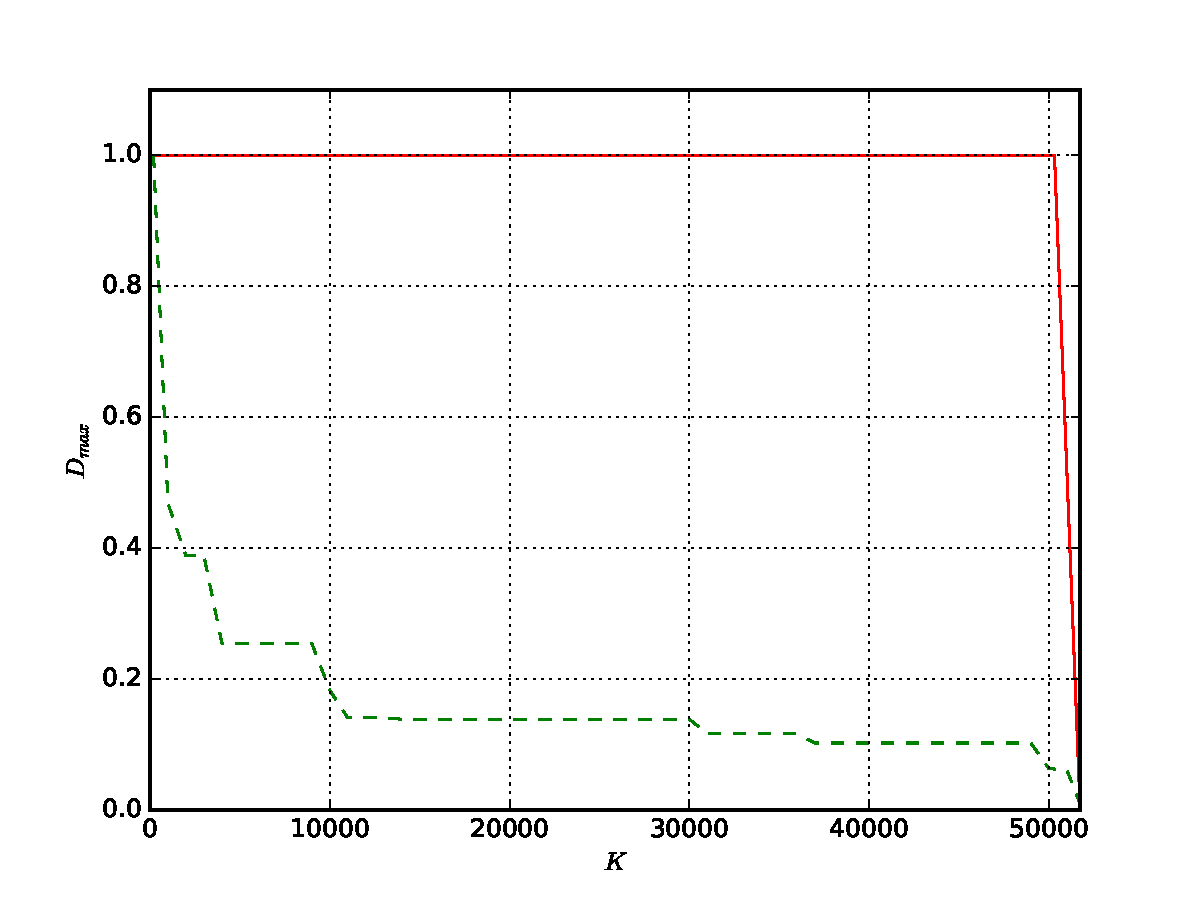
\includegraphics[width=.5\textwidth]{mixed_2d_max.pdf}}}
    \subfloat[\(D_{avg}\)]{
    \label{fig:avg_dev} {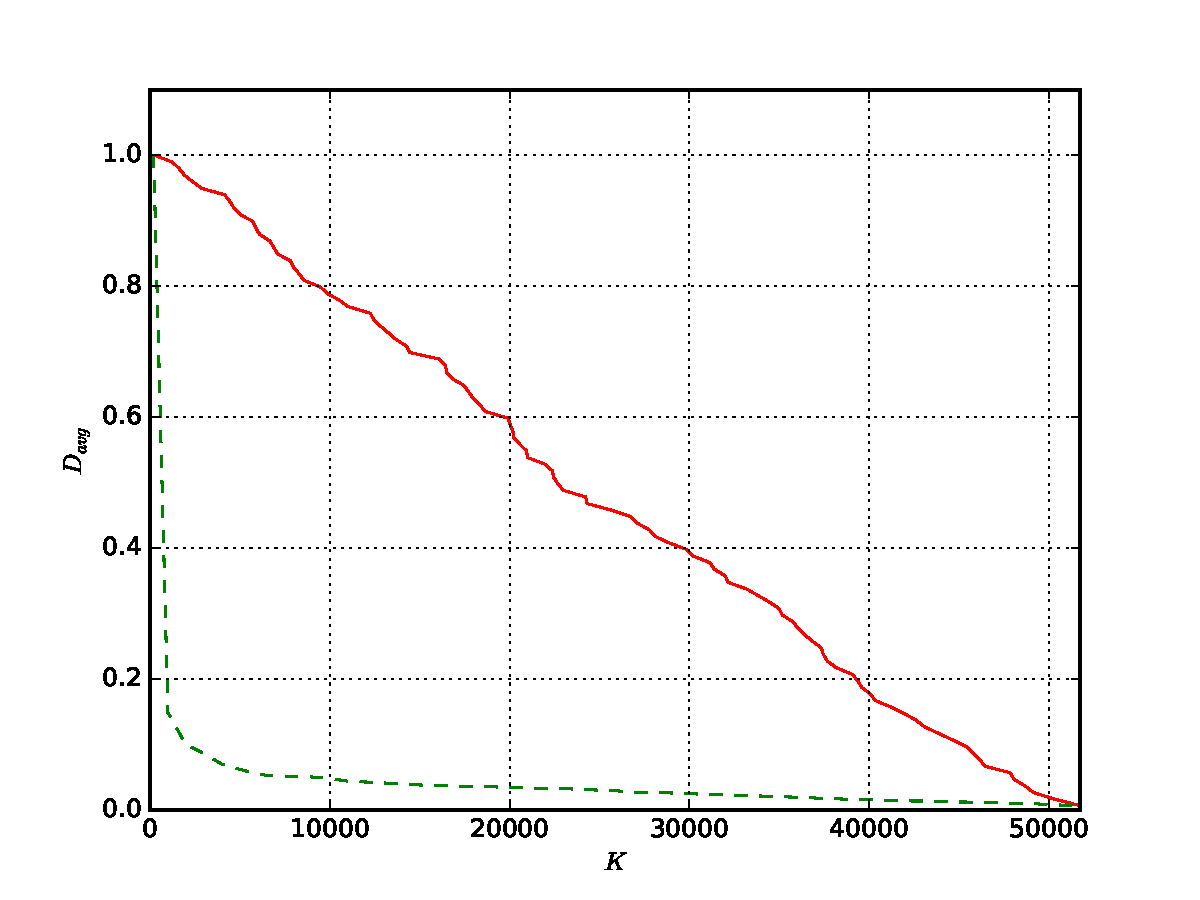
\includegraphics[width=.5\textwidth]{mixed_2d_avg.pdf}}}
    \caption{Динамика величин \(D_{avg}\) и \(D_{max}\) в процессе решения множества двухмерных задач,
    порождённых двумя разными генераторами GKLS и \(F_{GR}\)}
    \label{fig:devs_mixed}
\end{figure}

\subsection{Итоги}

В разделе \ref{sec:multi_algo} квалификационной работы была реализована поддержка нелинейных ограничений в алгоритме, решающeм
множество задач глобальной оптимизации в совокупности и распределяющего свои ресурсы так, чтобы
обеспечивать равномерную сходимость во всех задачах. Доказано теорема о достаточных условиях сходимости
полученного метода. Свойство равномерной сходимости проверено с помощью численного эксперимента.
Также в ходе численных экспериментов была оценена эффективность выполненной параллельной реализации метода и
показана эффективность совместного решения множества задач на примере получения Парето фронта в многокритериальной задаче с
нелинейными ограничениями.
